% Options for packages loaded elsewhere
\PassOptionsToPackage{unicode}{hyperref}
\PassOptionsToPackage{hyphens}{url}
%
\documentclass[
]{article}
\usepackage{amsmath,amssymb}
\usepackage{lmodern}
\usepackage{iftex}
\ifPDFTeX
  \usepackage[T1]{fontenc}
  \usepackage[utf8]{inputenc}
  \usepackage{textcomp} % provide euro and other symbols
\else % if luatex or xetex
  \usepackage{unicode-math}
  \defaultfontfeatures{Scale=MatchLowercase}
  \defaultfontfeatures[\rmfamily]{Ligatures=TeX,Scale=1}
\fi
% Use upquote if available, for straight quotes in verbatim environments
\IfFileExists{upquote.sty}{\usepackage{upquote}}{}
\IfFileExists{microtype.sty}{% use microtype if available
  \usepackage[]{microtype}
  \UseMicrotypeSet[protrusion]{basicmath} % disable protrusion for tt fonts
}{}
\makeatletter
\@ifundefined{KOMAClassName}{% if non-KOMA class
  \IfFileExists{parskip.sty}{%
    \usepackage{parskip}
  }{% else
    \setlength{\parindent}{0pt}
    \setlength{\parskip}{6pt plus 2pt minus 1pt}}
}{% if KOMA class
  \KOMAoptions{parskip=half}}
\makeatother
\usepackage{xcolor}
\usepackage[margin=1in]{geometry}
\usepackage{color}
\usepackage{fancyvrb}
\newcommand{\VerbBar}{|}
\newcommand{\VERB}{\Verb[commandchars=\\\{\}]}
\DefineVerbatimEnvironment{Highlighting}{Verbatim}{commandchars=\\\{\}}
% Add ',fontsize=\small' for more characters per line
\usepackage{framed}
\definecolor{shadecolor}{RGB}{248,248,248}
\newenvironment{Shaded}{\begin{snugshade}}{\end{snugshade}}
\newcommand{\AlertTok}[1]{\textcolor[rgb]{0.94,0.16,0.16}{#1}}
\newcommand{\AnnotationTok}[1]{\textcolor[rgb]{0.56,0.35,0.01}{\textbf{\textit{#1}}}}
\newcommand{\AttributeTok}[1]{\textcolor[rgb]{0.77,0.63,0.00}{#1}}
\newcommand{\BaseNTok}[1]{\textcolor[rgb]{0.00,0.00,0.81}{#1}}
\newcommand{\BuiltInTok}[1]{#1}
\newcommand{\CharTok}[1]{\textcolor[rgb]{0.31,0.60,0.02}{#1}}
\newcommand{\CommentTok}[1]{\textcolor[rgb]{0.56,0.35,0.01}{\textit{#1}}}
\newcommand{\CommentVarTok}[1]{\textcolor[rgb]{0.56,0.35,0.01}{\textbf{\textit{#1}}}}
\newcommand{\ConstantTok}[1]{\textcolor[rgb]{0.00,0.00,0.00}{#1}}
\newcommand{\ControlFlowTok}[1]{\textcolor[rgb]{0.13,0.29,0.53}{\textbf{#1}}}
\newcommand{\DataTypeTok}[1]{\textcolor[rgb]{0.13,0.29,0.53}{#1}}
\newcommand{\DecValTok}[1]{\textcolor[rgb]{0.00,0.00,0.81}{#1}}
\newcommand{\DocumentationTok}[1]{\textcolor[rgb]{0.56,0.35,0.01}{\textbf{\textit{#1}}}}
\newcommand{\ErrorTok}[1]{\textcolor[rgb]{0.64,0.00,0.00}{\textbf{#1}}}
\newcommand{\ExtensionTok}[1]{#1}
\newcommand{\FloatTok}[1]{\textcolor[rgb]{0.00,0.00,0.81}{#1}}
\newcommand{\FunctionTok}[1]{\textcolor[rgb]{0.00,0.00,0.00}{#1}}
\newcommand{\ImportTok}[1]{#1}
\newcommand{\InformationTok}[1]{\textcolor[rgb]{0.56,0.35,0.01}{\textbf{\textit{#1}}}}
\newcommand{\KeywordTok}[1]{\textcolor[rgb]{0.13,0.29,0.53}{\textbf{#1}}}
\newcommand{\NormalTok}[1]{#1}
\newcommand{\OperatorTok}[1]{\textcolor[rgb]{0.81,0.36,0.00}{\textbf{#1}}}
\newcommand{\OtherTok}[1]{\textcolor[rgb]{0.56,0.35,0.01}{#1}}
\newcommand{\PreprocessorTok}[1]{\textcolor[rgb]{0.56,0.35,0.01}{\textit{#1}}}
\newcommand{\RegionMarkerTok}[1]{#1}
\newcommand{\SpecialCharTok}[1]{\textcolor[rgb]{0.00,0.00,0.00}{#1}}
\newcommand{\SpecialStringTok}[1]{\textcolor[rgb]{0.31,0.60,0.02}{#1}}
\newcommand{\StringTok}[1]{\textcolor[rgb]{0.31,0.60,0.02}{#1}}
\newcommand{\VariableTok}[1]{\textcolor[rgb]{0.00,0.00,0.00}{#1}}
\newcommand{\VerbatimStringTok}[1]{\textcolor[rgb]{0.31,0.60,0.02}{#1}}
\newcommand{\WarningTok}[1]{\textcolor[rgb]{0.56,0.35,0.01}{\textbf{\textit{#1}}}}
\usepackage{graphicx}
\makeatletter
\def\maxwidth{\ifdim\Gin@nat@width>\linewidth\linewidth\else\Gin@nat@width\fi}
\def\maxheight{\ifdim\Gin@nat@height>\textheight\textheight\else\Gin@nat@height\fi}
\makeatother
% Scale images if necessary, so that they will not overflow the page
% margins by default, and it is still possible to overwrite the defaults
% using explicit options in \includegraphics[width, height, ...]{}
\setkeys{Gin}{width=\maxwidth,height=\maxheight,keepaspectratio}
% Set default figure placement to htbp
\makeatletter
\def\fps@figure{htbp}
\makeatother
\setlength{\emergencystretch}{3em} % prevent overfull lines
\providecommand{\tightlist}{%
  \setlength{\itemsep}{0pt}\setlength{\parskip}{0pt}}
\setcounter{secnumdepth}{-\maxdimen} % remove section numbering
\ifLuaTeX
  \usepackage{selnolig}  % disable illegal ligatures
\fi
\IfFileExists{bookmark.sty}{\usepackage{bookmark}}{\usepackage{hyperref}}
\IfFileExists{xurl.sty}{\usepackage{xurl}}{} % add URL line breaks if available
\urlstyle{same} % disable monospaced font for URLs
\hypersetup{
  pdftitle={Support and resampling metrics in parsimony analyses},
  pdfauthor={Daniel Yudi Miyahara Nakamura and Taran Grant},
  hidelinks,
  pdfcreator={LaTeX via pandoc}}

\title{Support and resampling metrics in parsimony analyses}
\author{Daniel Yudi Miyahara Nakamura and Taran Grant}
\date{2023-09-24}

\begin{document}
\maketitle

\hypertarget{preamble}{%
\section{1. Preamble}\label{preamble}}

Our aim is to test if bootstrap (BS) and jackknife (JN) predict support
(Goodman-Bremer, GB) in parsimony analyses. Our statistical analyses are
based on the protocol developed by Machado et al.~(2022)

\hypertarget{libraries}{%
\subsection{1.1 Libraries}\label{libraries}}

\begin{Shaded}
\begin{Highlighting}[]
\CommentTok{\# Load libraries}
\FunctionTok{library}\NormalTok{(canova)}
\FunctionTok{library}\NormalTok{(caret)}
\FunctionTok{library}\NormalTok{(devtools)}
\CommentTok{\#library(geoR)}
\FunctionTok{library}\NormalTok{(ggfortify)}
\FunctionTok{library}\NormalTok{(ggplot2)}
\FunctionTok{library}\NormalTok{(gridExtra)}
\FunctionTok{library}\NormalTok{(infotheo)}
\FunctionTok{library}\NormalTok{(knitr)}
\FunctionTok{library}\NormalTok{(MASS)}
\FunctionTok{library}\NormalTok{(mgcv)}
\FunctionTok{library}\NormalTok{(nlcor)}
\FunctionTok{detach}\NormalTok{(}\StringTok{"package:nlcor"}\NormalTok{) }\CommentTok{\# We detach this package once we stop using it}
\FunctionTok{library}\NormalTok{(quantreg)}
\FunctionTok{detach}\NormalTok{(}\StringTok{"package:quantreg"}\NormalTok{) }\CommentTok{\# We detach this package once we stop using it}
\FunctionTok{library}\NormalTok{(rcompanion)}
\FunctionTok{library}\NormalTok{(reshape2)}
\FunctionTok{library}\NormalTok{(scales)}
\FunctionTok{library}\NormalTok{(snow)}
\FunctionTok{library}\NormalTok{(splines)}
\FunctionTok{library}\NormalTok{(tidymv)}
\FunctionTok{library}\NormalTok{(tidyverse)}
\end{Highlighting}
\end{Shaded}

\hypertarget{datasets}{%
\subsection{1.2 Datasets}\label{datasets}}

\begin{Shaded}
\begin{Highlighting}[]
\CommentTok{\# Select working directory}
\FunctionTok{setwd}\NormalTok{(}\StringTok{"\textasciitilde{}/Downloads/supportParsimony\_R"}\NormalTok{)}

\CommentTok{\# Read data}
\NormalTok{rawData }\OtherTok{=} \FunctionTok{read\_csv}\NormalTok{(}\StringTok{"data.csv"}\NormalTok{)}
\end{Highlighting}
\end{Shaded}

\begin{verbatim}
## Rows: 794 Columns: 10
## -- Column specification --------------------------------------------------------
## Delimiter: ","
## chr (8): study, study_type, boot10, jack10, boot100, jack100, boot1000, jack...
## dbl (2): index, gb
## 
## i Use `spec()` to retrieve the full column specification for this data.
## i Specify the column types or set `show_col_types = FALSE` to quiet this message.
\end{verbatim}

\begin{Shaded}
\begin{Highlighting}[]
\NormalTok{rawData }\OtherTok{=} \FunctionTok{subset}\NormalTok{(rawData, }\SpecialCharTok{!}\FunctionTok{grepl}\NormalTok{(}\StringTok{"}\SpecialCharTok{\textbackslash{}\textbackslash{}}\StringTok{?"}\NormalTok{, boot1000)) }\CommentTok{\# remove unshared nodes}

\CommentTok{\# Treat variables as numeric}
\NormalTok{rawData}\SpecialCharTok{$}\NormalTok{gb }\OtherTok{=} \FunctionTok{as.numeric}\NormalTok{(rawData}\SpecialCharTok{$}\NormalTok{gb)}
\NormalTok{rawData}\SpecialCharTok{$}\NormalTok{boot1000 }\OtherTok{=} \FunctionTok{as.numeric}\NormalTok{(rawData}\SpecialCharTok{$}\NormalTok{boot1000)}
\NormalTok{rawData}\SpecialCharTok{$}\NormalTok{jack1000 }\OtherTok{=} \FunctionTok{as.numeric}\NormalTok{(rawData}\SpecialCharTok{$}\NormalTok{jack1000)}
\end{Highlighting}
\end{Shaded}

\hypertarget{exploratory-data-analysis}{%
\subsection{1.3 Exploratory data
analysis}\label{exploratory-data-analysis}}

\begin{Shaded}
\begin{Highlighting}[]
\CommentTok{\# Visualizing histograms}
\NormalTok{plot0 }\OtherTok{=} \FunctionTok{ggplot}\NormalTok{(rawData, }\FunctionTok{aes}\NormalTok{(}\AttributeTok{x =}\NormalTok{ gb)) }\SpecialCharTok{+}
  \FunctionTok{geom\_histogram}\NormalTok{(}\AttributeTok{binwidth =} \DecValTok{5}\NormalTok{, }\AttributeTok{fill =} \StringTok{"blue"}\NormalTok{, }\AttributeTok{color =} \StringTok{"black"}\NormalTok{, }\AttributeTok{alpha =} \FloatTok{0.7}\NormalTok{) }\SpecialCharTok{+}
  \FunctionTok{labs}\NormalTok{(}\AttributeTok{x =} \StringTok{"GB"}\NormalTok{, }\AttributeTok{y =} \StringTok{"Frequency"}\NormalTok{)}
\NormalTok{plot1 }\OtherTok{=} \FunctionTok{ggplot}\NormalTok{(rawData, }\FunctionTok{aes}\NormalTok{(}\AttributeTok{x =}\NormalTok{ boot1000)) }\SpecialCharTok{+}
  \FunctionTok{geom\_histogram}\NormalTok{(}\AttributeTok{binwidth =} \DecValTok{5}\NormalTok{, }\AttributeTok{fill =} \StringTok{"red"}\NormalTok{, }\AttributeTok{color =} \StringTok{"black"}\NormalTok{, }\AttributeTok{alpha =} \FloatTok{0.7}\NormalTok{) }\SpecialCharTok{+}
  \FunctionTok{labs}\NormalTok{(}\AttributeTok{x =} \StringTok{"Bootstrap"}\NormalTok{, }\AttributeTok{y =} \StringTok{"Frequency"}\NormalTok{)}
\NormalTok{plot2 }\OtherTok{=} \FunctionTok{ggplot}\NormalTok{(rawData, }\FunctionTok{aes}\NormalTok{(}\AttributeTok{x =}\NormalTok{ jack1000)) }\SpecialCharTok{+}
  \FunctionTok{geom\_histogram}\NormalTok{(}\AttributeTok{binwidth =} \DecValTok{5}\NormalTok{, }\AttributeTok{fill =} \StringTok{"darkgreen"}\NormalTok{, }\AttributeTok{color =} \StringTok{"black"}\NormalTok{, }\AttributeTok{alpha =} \FloatTok{0.7}\NormalTok{) }\SpecialCharTok{+}
  \FunctionTok{labs}\NormalTok{(}\AttributeTok{x =} \StringTok{"Jackknife"}\NormalTok{, }\AttributeTok{y =} \StringTok{"Frequency"}\NormalTok{)}
\FunctionTok{grid.arrange}\NormalTok{(plot0, plot1, plot2, }\AttributeTok{ncol =} \DecValTok{3}\NormalTok{)}
\end{Highlighting}
\end{Shaded}

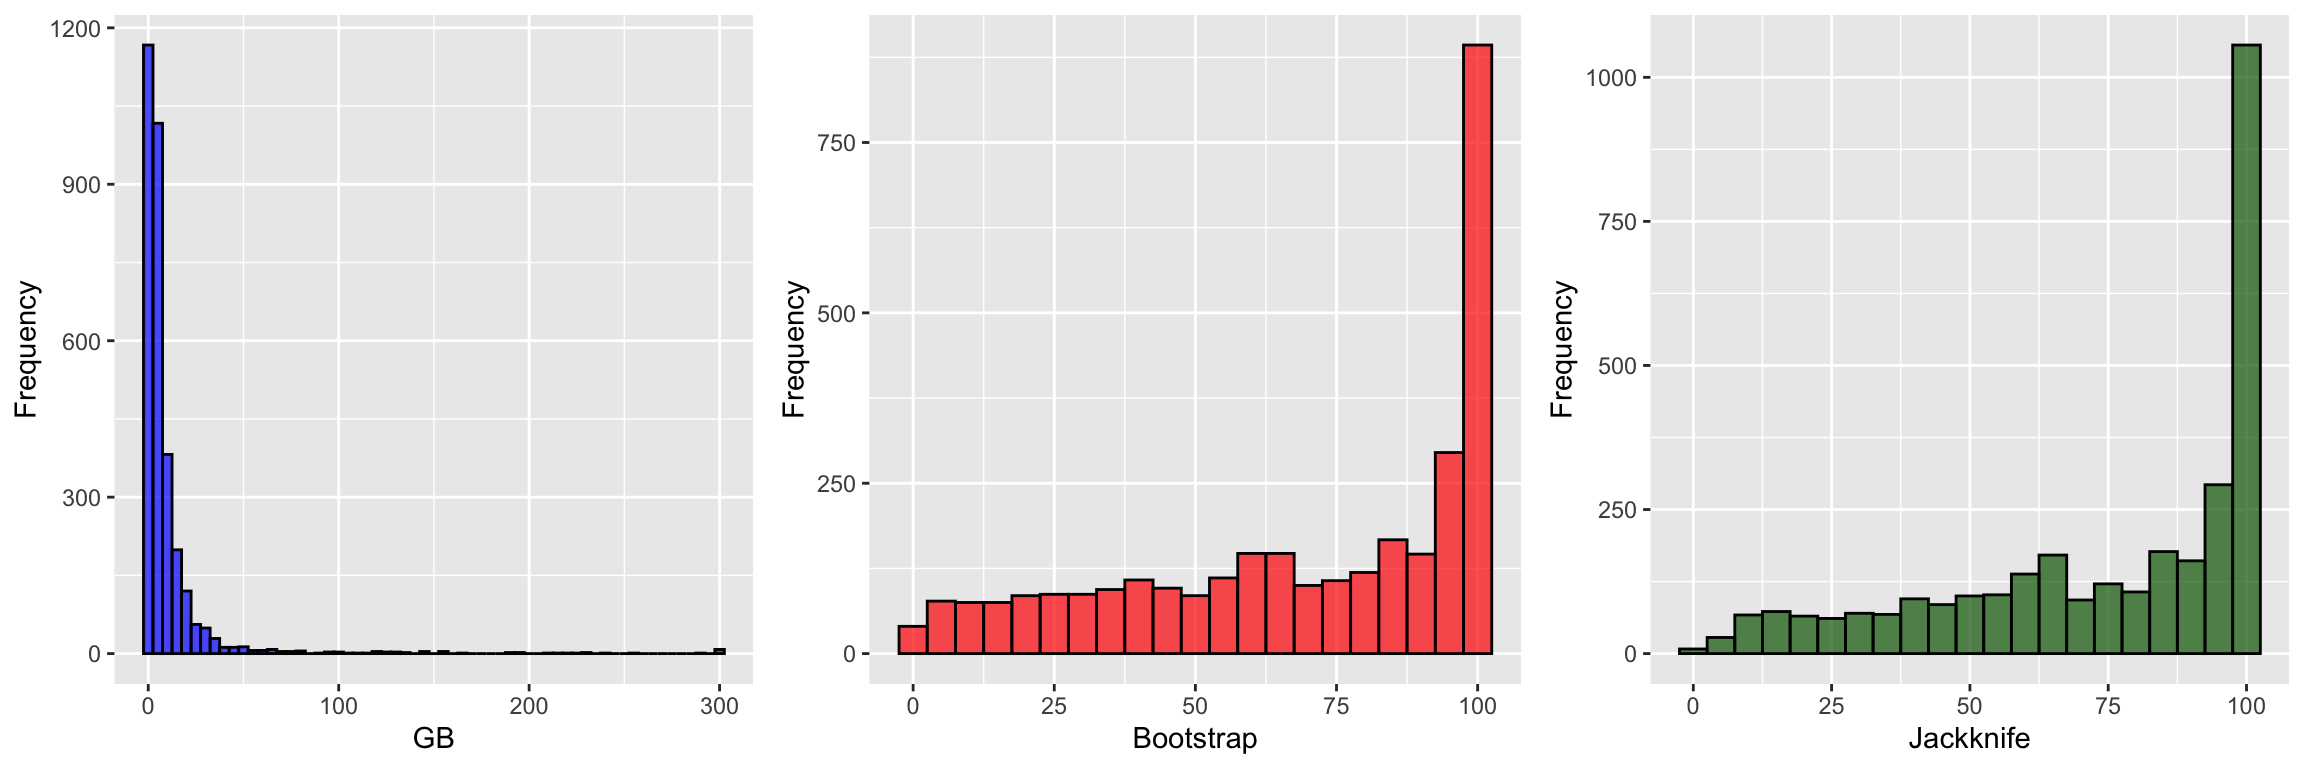
\includegraphics{supportParsimony_files/figure-latex/unnamed-chunk-2-1.pdf}

\begin{Shaded}
\begin{Highlighting}[]
\FunctionTok{rm}\NormalTok{(plot0, plot1, plot2)}
\end{Highlighting}
\end{Shaded}

\begin{Shaded}
\begin{Highlighting}[]
\CommentTok{\# Visualizing the raw data relationship}
\NormalTok{plot1 }\OtherTok{=} \FunctionTok{ggplot}\NormalTok{(rawData, }\FunctionTok{aes}\NormalTok{(}\AttributeTok{x =}\NormalTok{ boot1000, }\AttributeTok{y =}\NormalTok{ gb)) }\SpecialCharTok{+}
  \FunctionTok{geom\_point}\NormalTok{() }\SpecialCharTok{+}
  \FunctionTok{scale\_y\_continuous}\NormalTok{(}\AttributeTok{limits =} \FunctionTok{c}\NormalTok{(}\DecValTok{0}\NormalTok{, }\DecValTok{100}\NormalTok{)) }\SpecialCharTok{+}
  \FunctionTok{labs}\NormalTok{(}\AttributeTok{x =} \StringTok{"}\SpecialCharTok{\textbackslash{}n}\StringTok{Bootstrap"}\NormalTok{, }\AttributeTok{y =} \StringTok{"Goodman{-}Bremer}\SpecialCharTok{\textbackslash{}n}\StringTok{"}\NormalTok{)}
\NormalTok{plot2 }\OtherTok{=} \FunctionTok{ggplot}\NormalTok{(rawData, }\FunctionTok{aes}\NormalTok{(}\AttributeTok{x =}\NormalTok{ jack1000, }\AttributeTok{y =}\NormalTok{ gb)) }\SpecialCharTok{+}
  \FunctionTok{geom\_point}\NormalTok{() }\SpecialCharTok{+}
  \FunctionTok{scale\_y\_continuous}\NormalTok{(}\AttributeTok{limits =} \FunctionTok{c}\NormalTok{(}\DecValTok{0}\NormalTok{, }\DecValTok{100}\NormalTok{)) }\SpecialCharTok{+}
  \FunctionTok{labs}\NormalTok{(}\AttributeTok{x =} \StringTok{"}\SpecialCharTok{\textbackslash{}n}\StringTok{Jackknife"}\NormalTok{, }\AttributeTok{y =} \StringTok{"Goodman{-}Bremer}\SpecialCharTok{\textbackslash{}n}\StringTok{"}\NormalTok{)}
\FunctionTok{grid.arrange}\NormalTok{(plot1, plot2, }\AttributeTok{ncol =} \DecValTok{2}\NormalTok{)}
\end{Highlighting}
\end{Shaded}

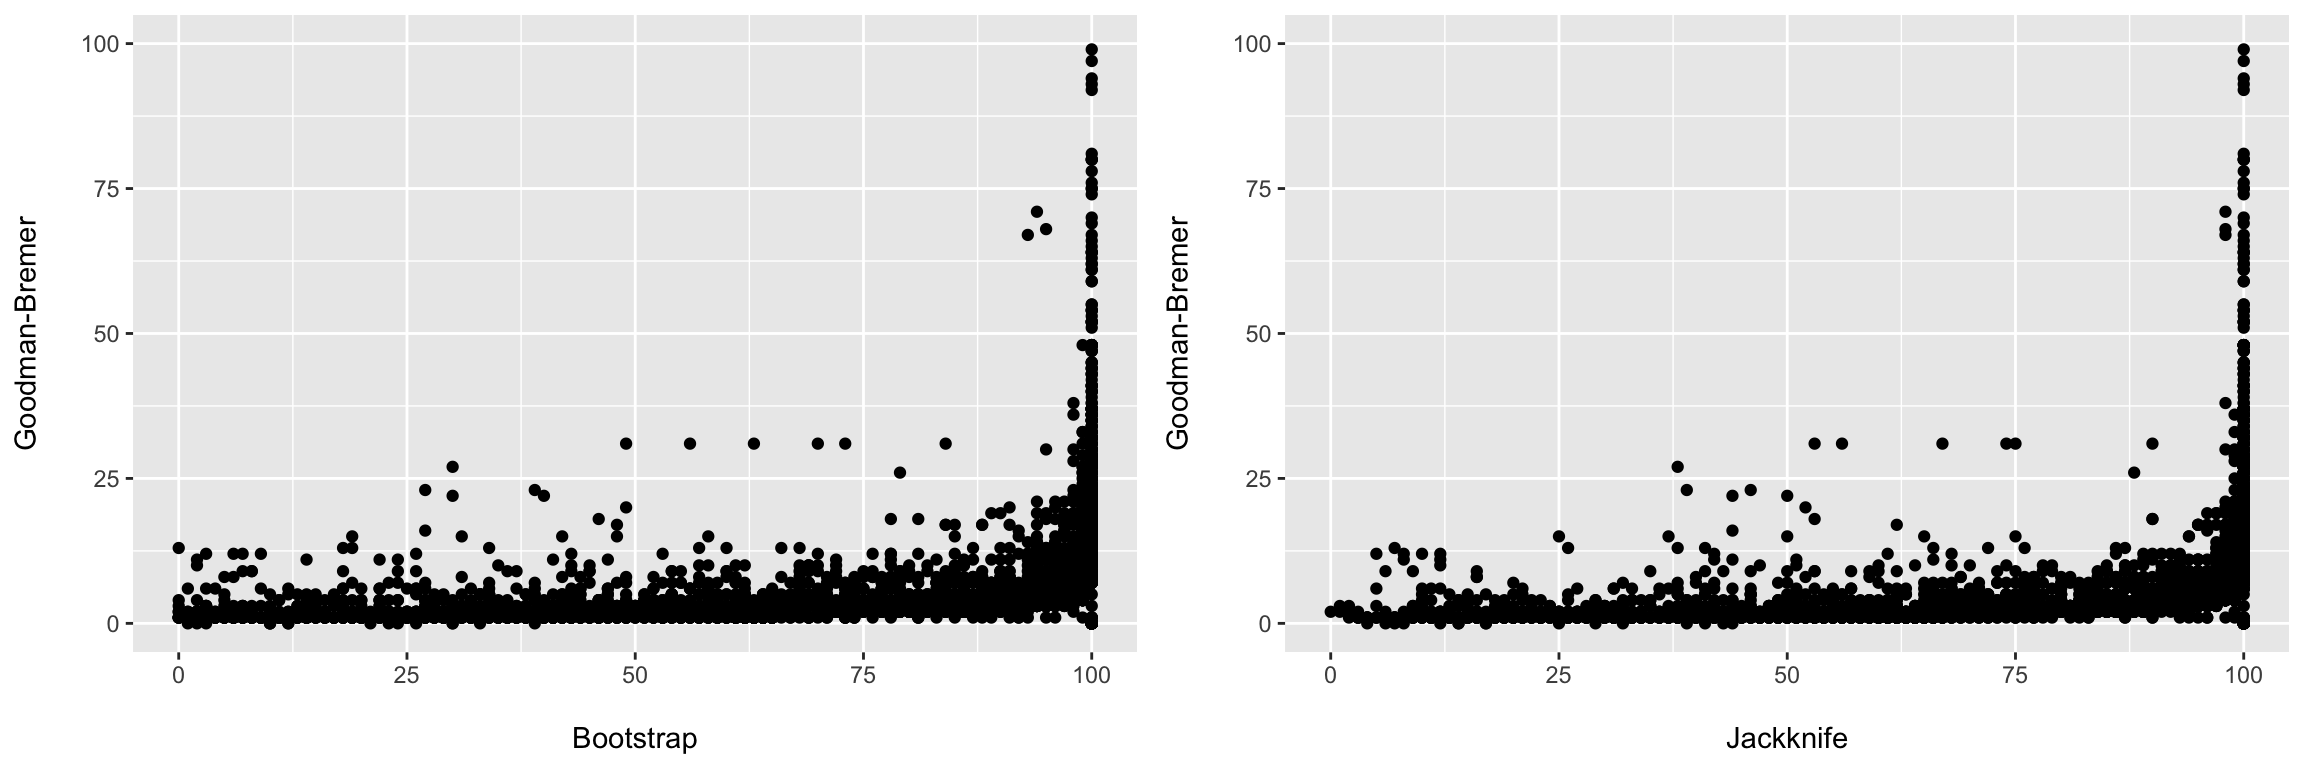
\includegraphics{supportParsimony_files/figure-latex/unnamed-chunk-3-1.pdf}

Based on the visualization plot above, the relationships between support
(GB) and resampling metrics (bootstrap and jackknife) do not seem
linear. Visually, neither bootstrap nor jackknife seem good predictors
of GB, but this must be better assessed with statistical tests (see
below).

\hypertarget{parametric-tests}{%
\section{2. Parametric tests}\label{parametric-tests}}

\hypertarget{non-parametric-tests}{%
\section{3. Non-parametric tests}\label{non-parametric-tests}}

\hypertarget{canova}{%
\subsection{CANOVA}\label{canova}}

\hypertarget{machine-learning-tests}{%
\section{4. Machine learning tests}\label{machine-learning-tests}}

We used machine learning techniques to assess overestimation and
underestimation of resampling metrics to support.

\hypertarget{conclusion}{%
\section{5. Conclusion}\label{conclusion}}

\hypertarget{references}{%
\section{6. References}\label{references}}

Machado, D.J., Marques, F.P.L., Jiménez‐Ferbans, L. \& Grant, T. (2022).
An empirical test of the relationship between the bootstrap and
likelihood ratio support in maximum likelihood phylogenetic analysis.
Cladistics, 38(3), 392-401.

\end{document}
